\section{Zielsetzung}
Das Ziel dieses Experimentes bestand darin, die Korpuskulartheorie von Licht nachzuweisen.
Außerdem wird das Planksche Wirkungsquantum bestimmt.

\section{Theorie}
\subsection{Der lichtelektrische Effekt}
Der Photoeffekt beschreibt den Vorgang, bei dem sich Elektronen durch Lichtbestrahlung von Metalloberflächen lösen.
Hierzu wird das Teilchenmodell von Licht aus der Quantendynamik zur Erklärung des Phänomens verwendet.
Dabei wird angenommen, dass das Licht als nicht weiter zerlegbare Energieportionen auftritt, die auch Photonen oder Lichtquanten genannt werden.


\subsection{Experimentelle Erkenntnisse}
Prinzipiell wird beim Photoeffekt ein im Vakuum befindliches Metall, welches als Photokathode bezeichnet wird, mit Licht bestrahlt und der dabei entstehende Strom gemessen.

\begin{figure}[h]
    \centering
    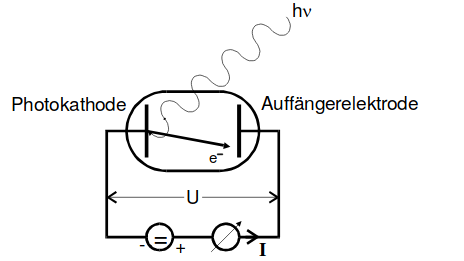
\includegraphics[height=5cm]{Theorie/Prinzip.png}
    \caption{Prinzipieller Versuchsaufbau.}
    \label{fig:prinzip}
\end{figure}

Im Gegensatz dazu den Photoeffekt mit dem Teilchenmodell zu erklären, könnte die theoretische Annahme getroffen werden, dass die Elektronen durch das schwingende elektromagnetische Feld des Lichts aus dem Metall gelöst werden.
So würde eine langfristige Bestrahlung mit genügend hoher Intensität jeder Wellenlänge bzw. jeder Frequenz Elektronen lösen und es könnte zu Resonanzfällen kommen.
Das Experiment liefert aber andere Beobachtungen.
Zunächst lässt sich sagen, dass die Zahl der pro Zeiteinheit gelösten Elektronen proportional zu der Lichtintensität ist.
Außerdem ist die Energie der gelösten Elektronen, die über den gemessenen Strom berechnet wird, linear in der Lichtfrequenz $\nu$ und unabhängig von der Lichtintensität.
Des Weiteren existiert eine minimale Frequenz, die auch als Grenzfrequenz bezeichnet wird, unter der keine Elektronen gelöst werden.\\

Unter der Annahme des Teilchenmodells nach Einstein sind diese Beobachtungen nun zu erklären.
Das Licht wird nicht mehr nur als Welle, in der die Energie über den Wellenraum gleichmäßig verteilt wäre, sondern auch als subatomares Teilchen von praktisch vernachlässigbarer Ausdehnung angenommen, bei dem die Energie portionsweise auf die Photonen verteilt ist.
Dies hat zur Folge, dass monochromatisches Licht somit nur Photonen gleicher Energien $h \nu$ aufwei\ss{}t.
Dieser Zusammenhang, dass die Photonenenergie proportional zur Lichtfrequenz ist, wird über die Energie der Elektronen und den damit verbundenen Strom folgendermaßen bestimmt.
Das Photon gibt seine Energie an das Elektron ab, wobei sich die Energie in die Austrittsarbeit $A_K$, die aufgebracht werden muss um das Elektron vom Feststoff zu lösen, und die kinetische Energie nach 
\begin{equation}
    \label{eqn:elektron}
    h \nu = \frac{m_0}{2} \; v_\text{max}^2 + A_K 
\end{equation}
aufteilt.
Der Photoeffekt tritt also nur für $h \nu \geq A_K$ auf.
Zusätzlich folgt aus Gleichung \ref{eqn:elektron}, dass die Energie der gelösten Elektronen nur linear in der Frequenz ist.
Des Weiteren ist die Lichtintensität proportional zur Zahl der auf das Metall auftreffenden Photonen pro Zeiteinheit, was die Intensitätsabhängigkeit der gelösten Elektronen pro Zeiteinheit erklärt.
 
\subsection{Die Gegenfeldmethode}
Bei der Gegenfeldmethode befinden sich im Vakuum zwei Elektroden, einerseits die Auffängerelektrode bzw. Anode und andererseits die Photokathode.
Zwischen den beiden Elektroden wird wie in Abbildung \ref{fig:prinzip} gezeigt eine Spannung angelegt, die die gelösten Elektronen auf dem Weg zur Anode entweder beschleunigt oder abbremst.
Da die angelegte Spannung die Elektronen meistens abbremsen soll, wird diese Gegenspannung auch $U_\text{geg}$ genannt und der Versuch als Gegenfeldmethode bezeichnet.
Somit gelangen nur Elektronen zur Anode, die eine genügend hohe kinetische Energie besitzen um das elektrische Potential zu überwinden.
Zur Bestimmung der kinetischen Energie der Elektronen wird die Gegenspannung so eingestellt, dass der Strom verschwindet und 
\begin{equation}
    \label{eqn:span}
    e_0 U_\text{geg} = \frac{m_0}{2} \;v_\text{max}^2.
\end{equation}
gilt.
Nach den Gleichungen \ref{eqn:elektron} und \ref{eqn:span} ergibt sich für die spannungsabhängige Energie der Photonen
\begin{equation}
    \label{eqn:photon}
    h \nu = e_0 U_\text{geg} + A_K.
\end{equation}

Daraus ergibt sich dann der lineare Zusammenhang zwischen Spannung und Lichtfrequenz mit
\begin{equation}
    \label{eqn:lin}
    U_\text{geg} = \frac{h \nu}{e_0} - \frac{A_K}{e_0}.
\end{equation}
Über diese Vorraussetzung lässt sich dann esperimentell das Planksche Wirkungsquantum $h$ bestimmen. \\

Der ebenfalls zu untersuchende Spannung-Strom-Zusammenhang wird in Abbildung \ref{fig:diagramm} augetragen.
Aus folgendem Grund erschwert sich die Messung der Grenzspannung $U_\text{geg}$.
Dies ergibt sich daraus, dass die Elektronen im Metall aufgrund des Pauli-Prinzips und des Spins unterschiedliche Energien besitzen, was anhand der Fermi-Diracschen-Wahrscheinlichkeitsverteilung gezeigt werden kann.
So erstreckt sich beim Temperaturnullpunkt $T = \SI{0}{K}$ das Energiespektrum der Leitungselektronen von 0 bis zur Fermie-Energie $\zeta$.\\
Bei Temperaturen $T > \SI{0}{K}$ können auch Elektronen mit höheren Energien als der Fermie-Energie auftreten.
So gibt es auch die geringe Möglichkeit, dass Elektronen bei endlichen Temperaturen eine Energie haben, die größer als $h \nu - A_K$ ist.
Dadurch erschwert sich die Messung der Grenzspannung $U_g$, weil sich für die hochenergetischen Elektronen die Grenzspannung verschiebt, da mehr Arbeit aufgebracht werden muss um diese abzubremsen.\\

Außerdem kann nicht gewährleistet werden, dass alle gelösten Elektronen die Auffängerelektrode erreichen und somit zum gemessenen Strom beitragen.
Das äu\ss{}ert sich im Spannung-Strom-Diagramm in Abbildung \ref{fig:diagramm} dadurch, dass  kontinuierlich Photostrom bereits bei $U < U_g$ deutlich und nichtlinear gegen null geht, und nicht erst bei $U_\text{geg} = U_g$.

\begin{figure}[h]
    \centering
    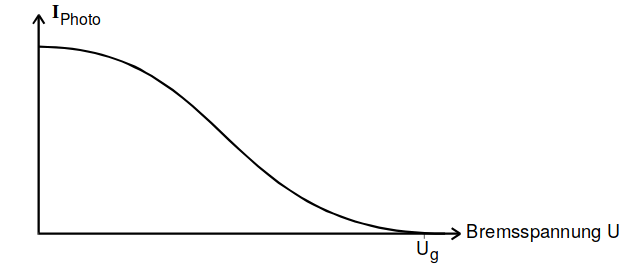
\includegraphics[height=5cm]{Theorie/Diagramm.png}
    \caption{.Experimentelle Kurve des Photostroms $I_\text{Photo}$ und der Gegenspannung $U_\text{geg}$ und Eintrag der Grenzspannung $U_g$}
    \label{fig:diagramm}
\end{figure}

Des Weiteren werden die Elektronen falls die Austrittsarbeit der Anode $A_A$ größer ist als die der Photokathode $A_K$, zusätzlich gebremst.
Dies wird in Abbildung \ref{fig:arbeit} so dargestellt, dass eine zusätzliche Beschleunigungsspannung nötig wäre damit Elektronen in die Anode eintreten könnten und ein Photostrom messbar wäre.

\begin{figure}[h]
    \centering
    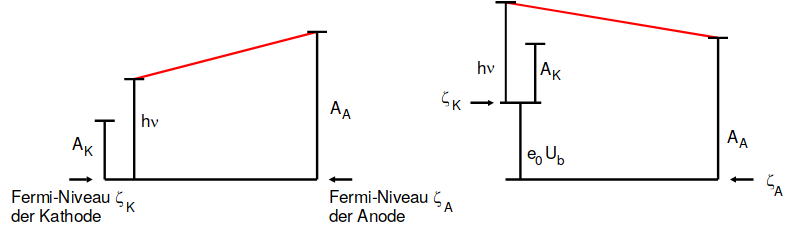
\includegraphics[height=4cm]{Theorie/Energie.png}
    \caption{Energieniveaus der Photo- und Auffangelektrode ohne (links) und mit (rechts) Beschleunigungsspannung.}
    \label{fig:arbeit}
\end{figure}

In der Umgebung von $U_g$ lässt sich der Zusammenhang zwischen der angelegten Gegenspannung und des Photostroms mit
\begin{equation}
    \label{eqn:prop}
    I_\text{Ph} \propto U_\text{geg}^2
\end{equation}
nähern.
Die Grenzspannung $U_g$ gibt dabei die Schnittstelle mit der Spannungsachse wieder.
